% ------------------------------------------------------------------------------ %
% The ?rst information LATEX needs to know when processing an input ?le is
% the type of document the author wants to create. This is speci?ed with the
% \documentclass command.
%
%   \documentclass[options]{class}
%
% Here class speci?es the type of document to be created.

\documentclass[a4paper,11pt]{article}

% The above command instructs LATEX to typeset the document as an article with
% a base font size of eleven points, printing on A4 paper.
% ------------------------------------------------------------------------------- %


% ------------------------------------------------------------------------------- %
% While writing your document, you will probably ?nd that there are some
% areas where basic LATEX cannot solve your problem. If you want to include
% graphics, coloured text or source code from a ?le into your document, you
% need to enhance the capabilities of LATEX. Such enhancements are called
% packages. Packages are activated with the
%
%   \usepackage[options]{package}
%
% command, where package is the name of the package and options is a list of
% keywords that trigger special features in the package.
%
% ATTENTION: IN ORDER TO ENABLE THE GREEK TYPESETTING YOU NEED TO INCLUDE IN YOUR
%            PREAMBLE SPECIFIC PACKAGES VIA THE USE OF THE \usepackage COMMAND.
%
%            THE SAME IS TRUE FOR SPECIFIC MATH FONTS ETC.


% * Activating Greek fonts in Latex
  \usepackage[english,greek]{babel} % the last language is the default

  %% > UNCOMMENT if your editor uses iso-8859-7 encoding for Greek (typical in Windows System).
  %\usepackage[iso-8859-7]{inputenc}

  %% > UNCOMMENT if your editor uses Unicode encoding for Greek (typical in POSIX Systems).
  \usepackage[utf8x]{inputenc}

  % One bad thing about the babel package is that it cannot discriminate explicitly between
  % Greek and Latin fonts, so you have to state commands in order to signify where the
  % Latin charecters begin and where they end and the Greek characters begin. For this
  % job the \latintext and \greektext commands exist. However Latex give you the versatility
  % to create wildcards for all of each commands and thus, to create alias with shorter
  % word length. Below we create the aliaces \lt and \gt for the \textlatin and \textgreek
  % commands respectively.

  \newcommand{\lt}{\latintext}
  \newcommand{\gt}{\greektext}


% * Math packages
 % \usepackage{amsthm}
  \usepackage{amsmath}
 % \usepackage{amssymb}

% * graphics package
  \usepackage[pdftex]{graphicx} % remove the 'pdftex' option if not PDFLatex is used.

% * verbatim writing package (mainly used to import program's code)
  \usepackage{verbatim}

% Used to prevent errors while using >{\em} for array columns
  \usepackage{array}

% Used for the final array at exercise 4
  \usepackage{multirow}

% Used to get greek letter support in enumeration
  \usepackage{moreenum}

% Used for bold font in enumeration
  \usepackage{enumitem}

% ------------------------------------------------------------------------------- %


% ------------------------------------------------------------------------------- %
% Here we set the title, the author and the date of our document.
%
% * Setting the title of the document
  \title{Προαιρετική εργασία \lt LaTeX} % Put your own title here

% * Setting the author or authors of the document
  \author{Ονοματεπώνυμο: Στέφανος Καραμπέρας  \\  ΑΕΜ: 2910}       % Put your own Name and AEM here

% * Setting the date of the document
  \date{\today}                                      % Put a specific date here
% ------------------------------------------------------------------------------- %


% =============================================================================== %
% ||                       HERE WE BEGIN OUR DOCUMENT                          || %
% =============================================================================== %
\begin{document}

% *** We are now inside the document everything from now on is VISIBLE!!! *** %

% Command that prints the title of your document
\maketitle

\section{Άσκηση 1 (Λύση)}
	
	\begin{center}
		\emph{{\tiny Α}{\scriptsize Β}{\footnotesize Γ}{\small Δ}{\normalsize Ε}{\large Ζ}{\Large Η}{\LARGE Θ}{\huge Ι}{\huge κ}{\LARGE λ}{\Large μ}{\large ν}{\normalsize ξ}{\small ο}{\footnotesize π}{\scriptsize ρ}{\tiny ς}}
	\end{center}

\vspace{20pt}

\section{Άσκηση 2 (Λύση)}

	\begin{center}	
		\lt
		\textit{Normal Italics \textbf{Bold\\}}
		{E}\textit{mphasized \underline{Underlined}}
	\end{center}

\section{Άσκηση 3 (Λύση)}
	
	\begin{equation*}
	a^2 + b^2 = c^2
	\end{equation*}
	\begin{equation*}
	e^{i\pi} = -1
	\end{equation*}
	\begin{equation*}
	\pi = \frac{c}{d}
	\end{equation*}
	\begin{equation*}
	\dfrac{d}{dx}\int_{a}^{x} f(s) ds = f(x)
	\end{equation*}
	\begin{equation*}
	f(x) = \sum_{i=0}^{\infty } {\dfrac{f^{(i)}(0)}{i!} x^i }
	\end{equation*}
	\begin{equation*}
	\textbf{\lt{Ax = b}}
	\end{equation*}
	\begin{equation*}
	||{x+y}||\leq||x||+||y||
	\end{equation*}
	
	\quad
	
	\begin{equation}
	\textbf{I} = 
	\begin{pmatrix}
	1&0&0&0 \\
	0&1&0&0 \\
	0&0&1&0 \\
	0&0&0&1 \\
	\end{pmatrix}
	\end{equation}
	
	\quad
	
	\begin{equation}
	\textbf{I} = 
	\begin{bmatrix}
	1&0&0&0 \\
	0&1&0&0 \\
	0&0&1&0 \\
	0&0&0&1 \\
	\end{bmatrix}
	\end{equation}
	
	\quad
	
	\begin{equation}
	\textbf{I} =
	\begin{Bmatrix} 
	1&0&0&0 \\
	0&1&0&0 \\
	0&0&1&0 \\
	0&0&0&1 \\
	\end{Bmatrix},\quad
	\textbf{I} =
	\begin{vmatrix} 
	1&0&0&0 \\
	0&1&0&0 \\
	0&0&1&0 \\
	0&0&0&1 \\
	\end{vmatrix},\quad
	\textbf{I} =
	\begin{Vmatrix} 
	1&0&0&0 \\
	0&1&0&0 \\
	0&0&1&0 \\
	0&0&0&1 \\
	\end{Vmatrix}
	\end{equation}

\vspace{20pt}

\section{Άσκηση 4 (Λύση)}
		
	\begin{table}[!h]
	\centering
	\begin{tabular}{ >{\em}l >{\em}c >{\em}c }
	Τέφας & 2 & 3 \\ 
	Πήτας & 5 & 6 \\ 
	Λάσκαρης & 8 & 9 \\ 
	\end{tabular}
	\end{table}	

	\begin{table}[!h]
	\centering
	\begin{tabular}{ | >{\em}l | >{\em}c | >{\em}c | }
	Κοτρόπουλος & 2 & 3 \\
	Πήτας & 5 & 6 \\ 
	Νικολαίδης & 8 & 9 \\ 
	\end{tabular}
	\end{table}		
	
	\begin{table}[!h]
	\centering
	\begin{tabular}{|>{\em}c|>{\em}c|>{\em}c|} \hline
	1 & 2 & 3 \\ \hline
	4 & 5 & 6 \\ \hline
	7 & 8 & 9 \\ \hline
	\end{tabular}
	\end{table}
	
	\begin{table}[!h]
	\centering
	\begin{tabular}{|>{\em}c|>{\em}c|>{\em}c|} \hline
	1 & 2 & 3 \\ \hline
	4 & 5 & 6 \\ \hline
	7 & 8 & 9 \\ \hline
	\end{tabular}
	\end{table}
	
	\begin{tabular}{ |>{\em}l|>{\em}l|>{\em}l| }
	\hline
	\multicolumn{3}{ |>{\em}c| }{Μέλη ΔΕΠ Πληροφορικής} \\
	\hline
	Λέκτορες & \lt VD & Δραζιώτης Κωνσταντίνος \\ \hline
	\multirow{2}{*}{Επίκουροι} 
          & \lt LN & Λάσκαρης Νικόλαος \\
	 & \lt TG & Τσουμάκας Γρηγόριος \\ \hline
	\multirow{3}{*}{Αναπληρωτές} 
	 & \lt TA & Τέφας Αναστάσιος \\
	 & \lt PN & Πλέρος Νίκος \\
	 & \lt PA & Παπαδόπουλος Απόστολος \\ \hline
	\multirow{3}{*}{Καθηγητές} 
	& \lt KC & Κοτρόπουλος Κωνσταντίνος \\
	& \lt PI & Πήτας Ιωάννης \\
	& \lt VI & Βλαχάβας Ιωάννης \\ 
	
	\hline
	\end{tabular}

\vspace{20pt}

\section{Άσκηση 5 (Λύση)}
		
	\begin{itemize}  
	\item \textit{Τέφας}
	\item \textit{Μπουζάς}
	\item \textit{Μπρούζα}
	\item \textit{Λάσκαρης}
	\item \textit{Κοτρόπουλος}
	\item \textit{Πήτας}
	\item \textit{Νικολαΐδης}	
	\end{itemize}	
	
	\begin{enumerate}  
	\item \textit{Τέφας}
	\item \textit{Μπουζάς}
	\item \textit{Μπρούζα}
	\item \textit{Λάσκαρης}
	\item \textit{Κοτρόπουλος}
	\item \textit{Πήτας}
	\item \textit{Νικολαΐδης}	
	\end{enumerate}	
	
	\begin{enumerate}[label=\textbf(\greek*)]
	\item \textit{Τέφας}
	\item \textit{Μπουζάς}
	\item \textit{Μπρούζα}
	\item \textit{Λάσκαρης}
	\item \textit{Κοτρόπουλος}
	\item \textit{Πήτας}
	\item \textit{Νικολαΐδης}	
	\end{enumerate}	

\vspace{20pt}

\section{Άσκηση 6 (Λύση)}



	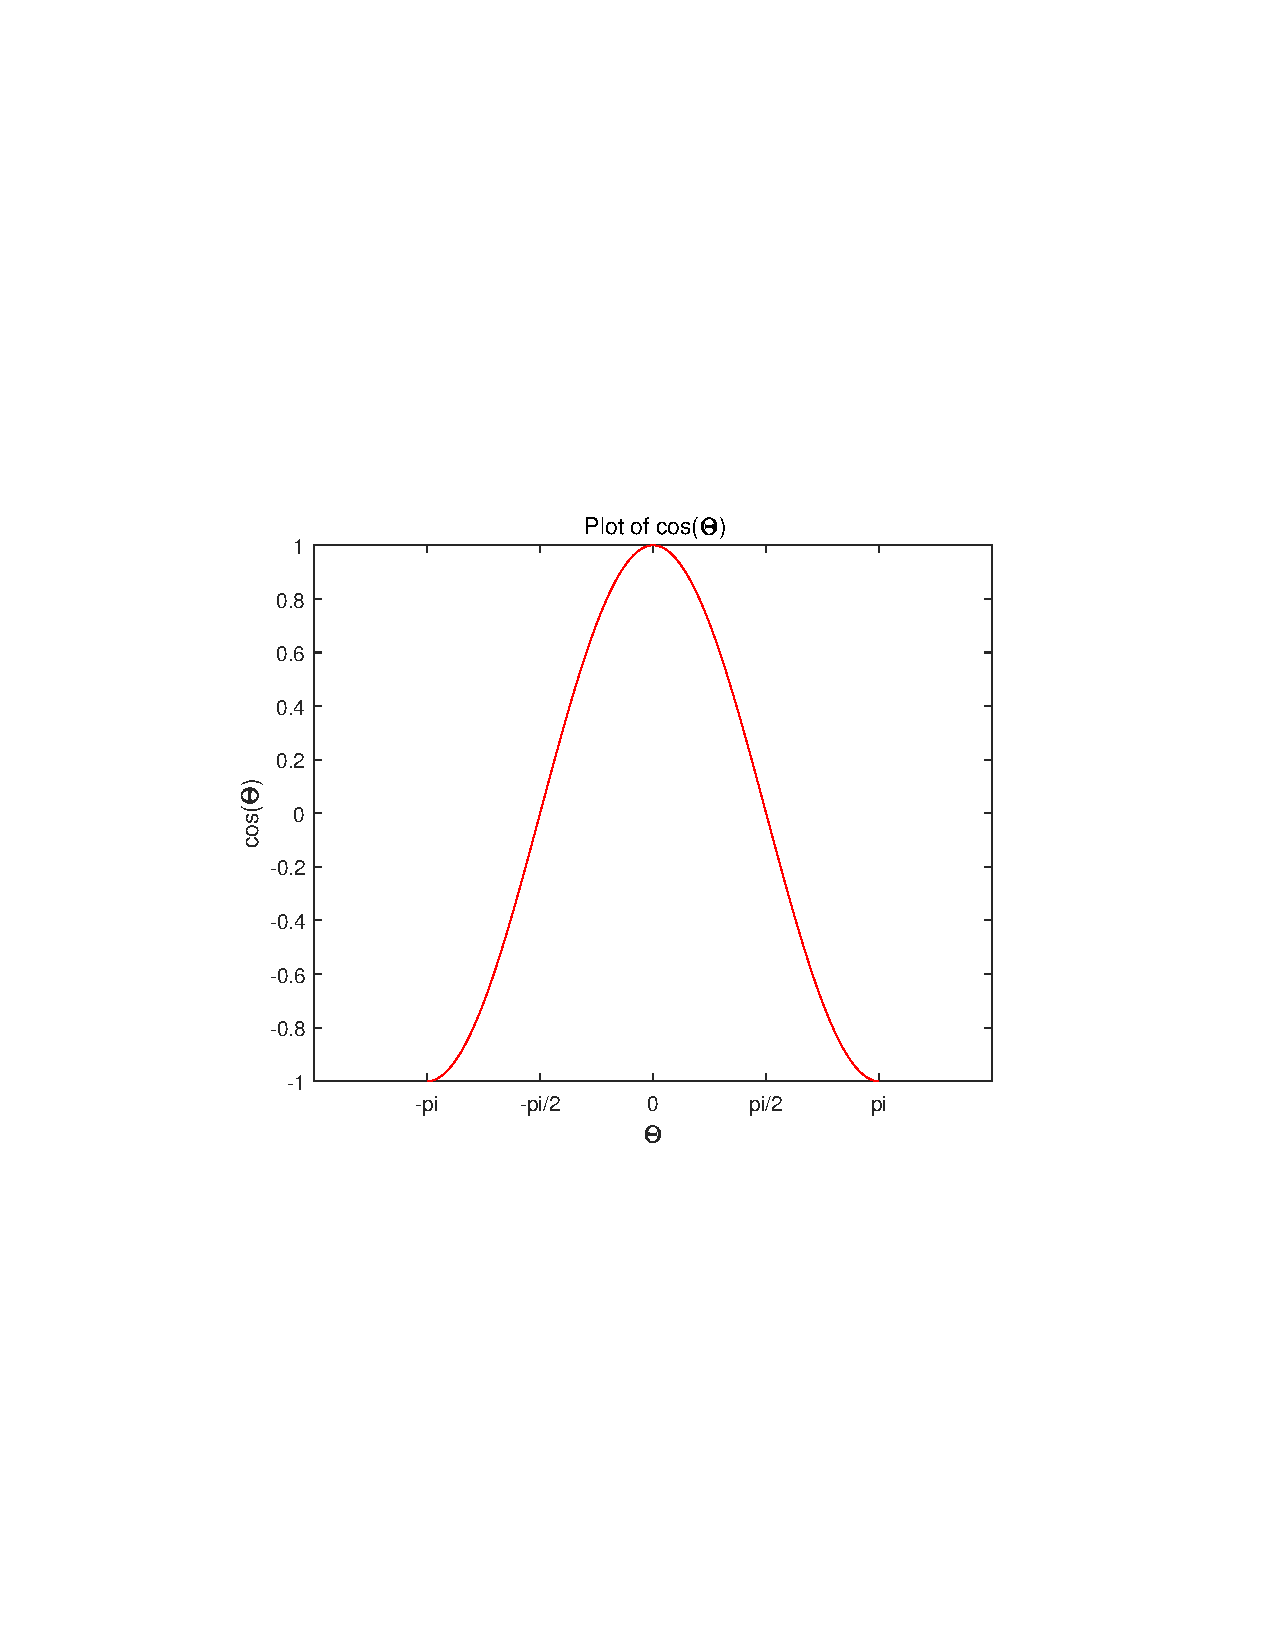
\includegraphics[width=\linewidth]{plot1}
	
	\vspace{10pt}
	
	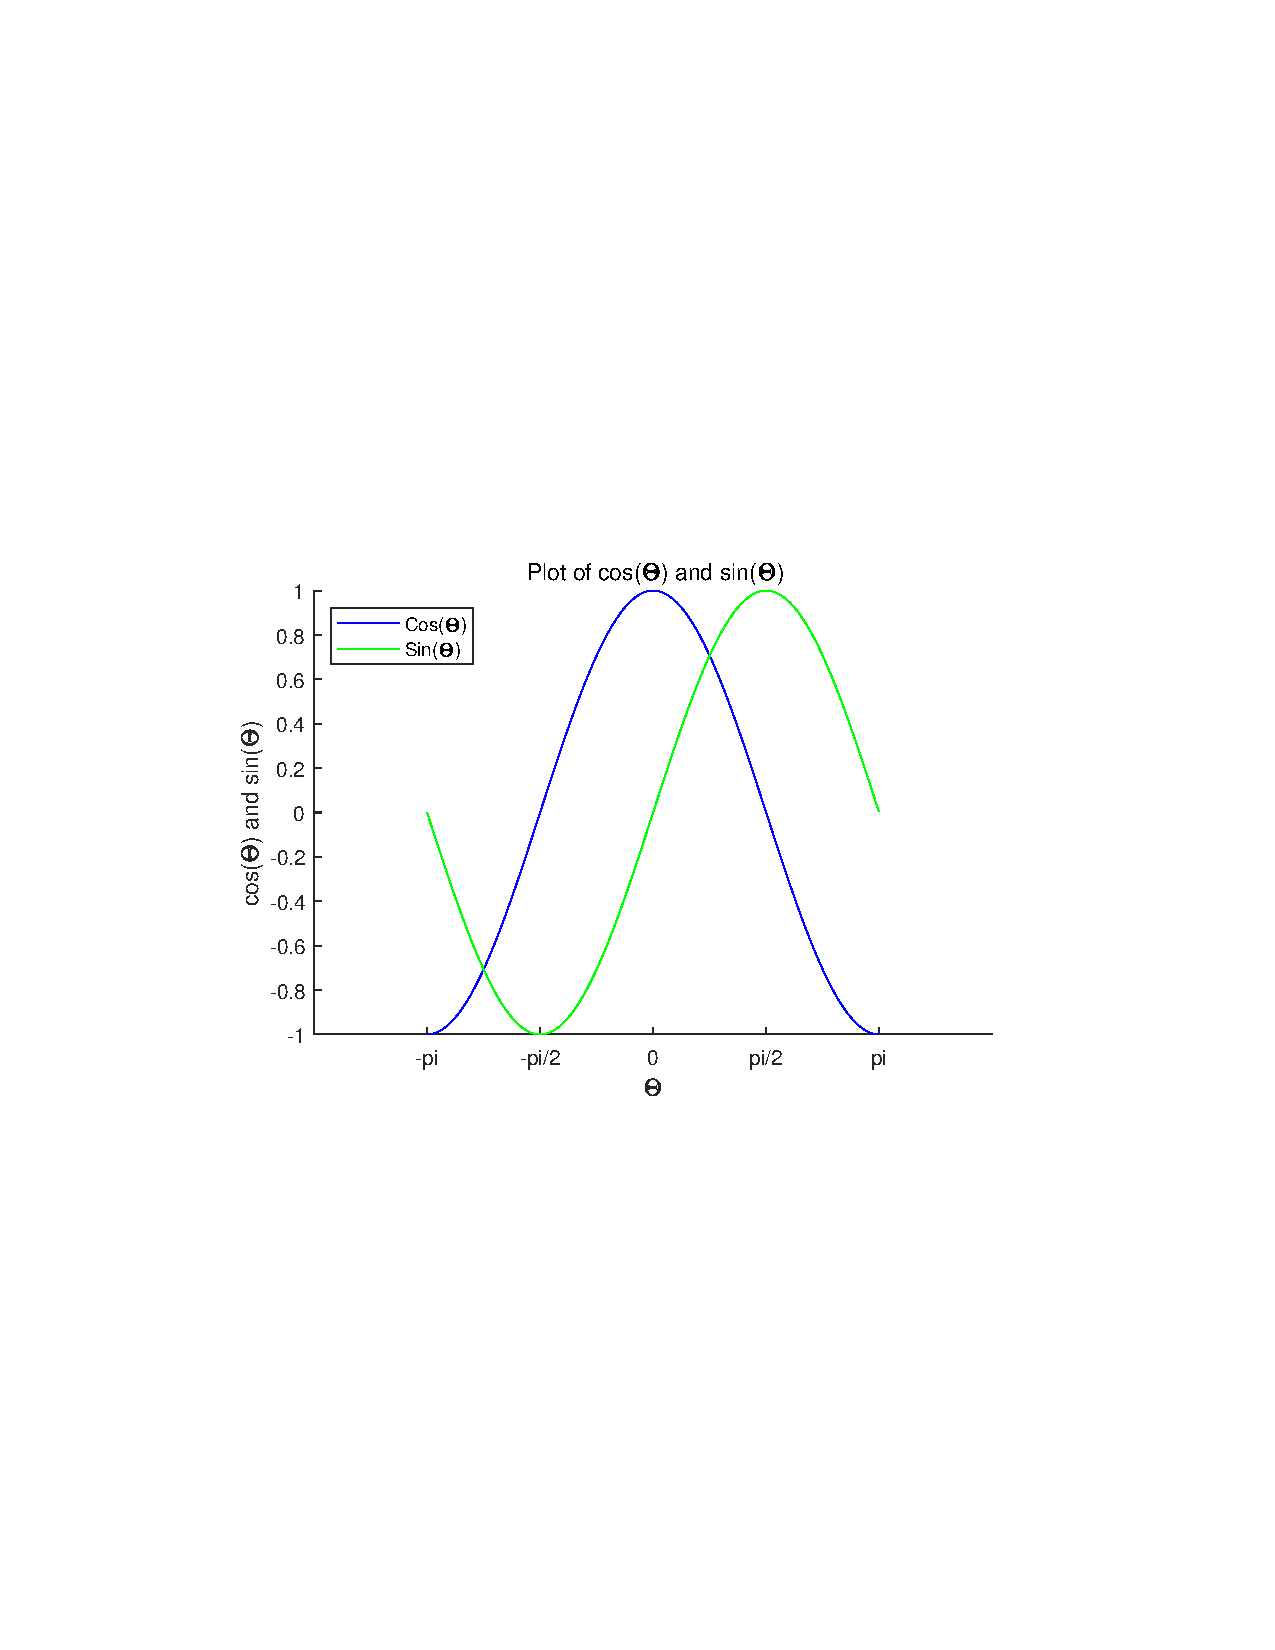
\includegraphics[width=\linewidth]{plot2}

% =============================================================================== %
% ||                       HERE WE END OUR DOCUMENT                          || %
% =============================================================================== %
\end{document}
